% GENERATED FILE - do not hand-edit.
% Source of truth: data/calculus-reviewed/c-7.json in the zenith-website repo.
% Regenerate with: python3 scripts/build_calculus_tex.py
\documentclass[11pt]{article}
\usepackage[utf8]{inputenc}
\usepackage[T1]{fontenc}
\usepackage{amsmath,amssymb}
\usepackage{graphicx}
\usepackage[margin=1in]{geometry}
\graphicspath{{../..//}}
\setlength{\parindent}{0pt}
\setlength{\parskip}{0.6em}
\begin{document}
\section*{Chapter 7: Application of Integration to Geometry --- Practice Exercises C7}

\bigskip\noindent\textbf{A1.}\ Find the area bounded by $y=x^2$, $y=0$, $x=-1$, and $x=2$.
\begin{list}{}{\setlength{\leftmargin}{3em}\setlength{\labelwidth}{2.5em}\setlength{\itemsep}{0pt}\setlength{\topsep}{2pt}}
\item[(A)] $11/3$
\item[(B)] $7/3$
\item[(C)] $3$
\item[(D)] $5$
\end{list}

\bigskip\noindent\textbf{A2.}\ Find the area between $y=x^2-3$ and $y=1$.
\begin{list}{}{\setlength{\leftmargin}{3em}\setlength{\labelwidth}{2.5em}\setlength{\itemsep}{0pt}\setlength{\topsep}{2pt}}
\item[(A)] $8/3$
\item[(B)] $32$
\item[(C)] $32/3$
\item[(D)] $16/3$
\end{list}

\bigskip\noindent\textbf{A3.}\ Find the area bounded by $x=y^2-1$ and the $y$-axis.
\begin{list}{}{\setlength{\leftmargin}{3em}\setlength{\labelwidth}{2.5em}\setlength{\itemsep}{0pt}\setlength{\topsep}{2pt}}
\item[(A)] $4/3$
\item[(B)] $2/3$
\item[(C)] $8/3$
\item[(D)] $1/2$
\end{list}

\bigskip\noindent\textbf{A4.}\ Find the area between $y^2=x$ and $x+y=2$.
\begin{center}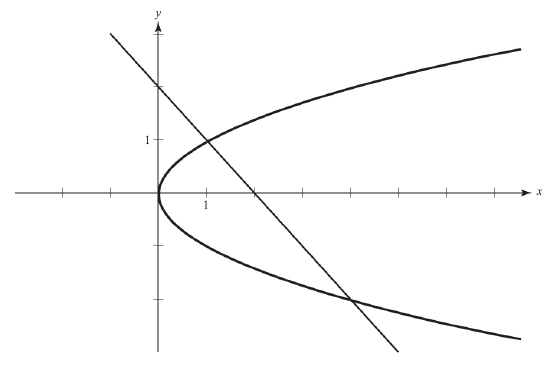
\includegraphics[width=0.6\linewidth]{data/calculus-figures/c7-a4.png}\end{center}
\begin{list}{}{\setlength{\leftmargin}{3em}\setlength{\labelwidth}{2.5em}\setlength{\itemsep}{0pt}\setlength{\topsep}{2pt}}
\item[(A)] $15/2$
\item[(B)] $3/2$
\item[(C)] $21/6$
\item[(D)] $9/2$
\end{list}

\bigskip\noindent\textbf{A5.}\ Find the area bounded by $y=4/(x^2+4)$, the $x$-axis, and $x=-2,2$.
\begin{list}{}{\setlength{\leftmargin}{3em}\setlength{\labelwidth}{2.5em}\setlength{\itemsep}{0pt}\setlength{\topsep}{2pt}}
\item[(A)] $\pi/4$
\item[(B)] $\pi/2$
\item[(C)] $2\pi$
\item[(D)] $\pi$
\end{list}

\bigskip\noindent\textbf{A6.}\ Find the area between $x=y^2-5y$ and $x=3y-y^2$.
\begin{center}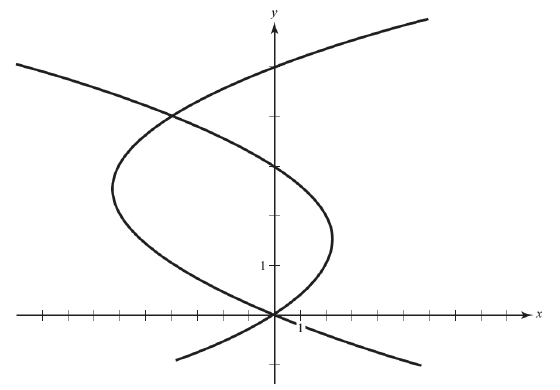
\includegraphics[width=0.6\linewidth]{data/calculus-figures/c7-a6.png}\end{center}
\begin{list}{}{\setlength{\leftmargin}{3em}\setlength{\labelwidth}{2.5em}\setlength{\itemsep}{0pt}\setlength{\topsep}{2pt}}
\item[(A)] $32/3$
\item[(B)] $139/6$
\item[(C)] $64/3$
\item[(D)] $128/3$
\end{list}

\bigskip\noindent\textbf{A7.}\ Find the area between $y=2/x$ and $x+y=3$.
\begin{list}{}{\setlength{\leftmargin}{3em}\setlength{\labelwidth}{2.5em}\setlength{\itemsep}{0pt}\setlength{\topsep}{2pt}}
\item[(A)] $1/2-2\ln2$
\item[(B)] $3/2$
\item[(C)] $1/2-\ln4$
\item[(D)] $3/2-\ln4$
\end{list}

\bigskip\noindent\textbf{A8.}\ Find the first-quadrant area bounded below by the $x$-axis and above by $y=\sin x$ and $y=\cos x$.
\begin{list}{}{\setlength{\leftmargin}{3em}\setlength{\labelwidth}{2.5em}\setlength{\itemsep}{0pt}\setlength{\topsep}{2pt}}
\item[(A)] $2-\sqrt2$
\item[(B)] $2+\sqrt2$
\item[(C)] $2$
\item[(D)] $\sqrt2$
\end{list}

\bigskip\noindent\textbf{A9.}\ Find the area above $y=\cos x$ and below $y=\sin x$ for $\pi/4\le x\le5\pi/4$.
\begin{list}{}{\setlength{\leftmargin}{3em}\setlength{\labelwidth}{2.5em}\setlength{\itemsep}{0pt}\setlength{\topsep}{2pt}}
\item[(A)] $2\sqrt2$
\item[(B)] $2/\sqrt2$
\item[(C)] $2(\sqrt2-1)$
\item[(D)] $2(\sqrt2+1)$
\end{list}

\bigskip\noindent\textbf{A10.}\ Find the area bounded by $y=\cot x$, $x=\pi/4$, and the $x$-axis.
\begin{list}{}{\setlength{\leftmargin}{3em}\setlength{\labelwidth}{2.5em}\setlength{\itemsep}{0pt}\setlength{\topsep}{2pt}}
\item[(A)] $\ln2$
\item[(B)] $\tfrac12\ln\tfrac12$
\item[(C)] $1$
\item[(D)] $\tfrac12\ln2$
\end{list}

\bigskip\noindent\textbf{A11.}\ Find the total area bounded by $y=x^3-2x^2-3x$ and the $x$-axis.
\begin{list}{}{\setlength{\leftmargin}{3em}\setlength{\labelwidth}{2.5em}\setlength{\itemsep}{0pt}\setlength{\topsep}{2pt}}
\item[(A)] $28/3$
\item[(B)] $79/6$
\item[(C)] $45/4$
\item[(D)] $71/6$
\end{list}

\bigskip\noindent\textbf{A12.}\ Find the total area bounded by $x=y^3-y$ and $x=3y$.
\begin{center}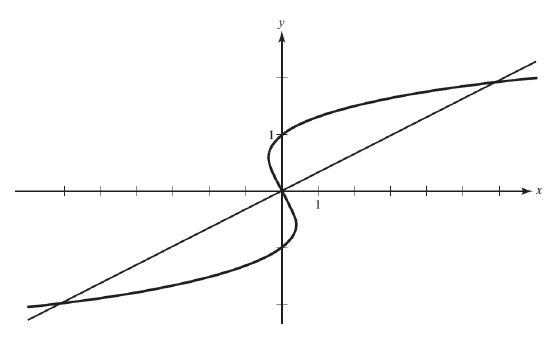
\includegraphics[width=0.6\linewidth]{data/calculus-figures/c7-a12.png}\end{center}
\begin{list}{}{\setlength{\leftmargin}{3em}\setlength{\labelwidth}{2.5em}\setlength{\itemsep}{0pt}\setlength{\topsep}{2pt}}
\item[(A)] $4$
\item[(B)] $16/3$
\item[(C)] $8$
\item[(D)] $16$
\end{list}

\bigskip\noindent\textbf{A13.}\ Find the area bounded by $y=e^x$, $y=2$, and the $y$-axis.
\begin{list}{}{\setlength{\leftmargin}{3em}\setlength{\labelwidth}{2.5em}\setlength{\itemsep}{0pt}\setlength{\topsep}{2pt}}
\item[(A)] $3-e$
\item[(B)] $e^2+1$
\item[(C)] $2\ln2-1$
\item[(D)] $2\ln2-3$
\end{list}

\bigskip\noindent\textbf{A14.}\ The area enclosed by $y^2=x(1-x)$ is given by
\begin{list}{}{\setlength{\leftmargin}{3em}\setlength{\labelwidth}{2.5em}\setlength{\itemsep}{0pt}\setlength{\topsep}{2pt}}
\item[(A)] $2\int_0^1x\sqrt{1-x}\,dx$
\item[(B)] $2\int_0^1\sqrt{x-x^2}\,dx$
\item[(C)] $4\int_0^1\sqrt{x-x^2}\,dx$
\item[(D)] $\pi$
\end{list}

\bigskip\noindent\textbf{A15.}\ The figure shows $y=x^3$ and a rectangle with bottom vertices $(0,0)$ and $(c,0)$ and upper-right vertex on the curve. What is the ratio of the rectangle's area to its shaded part above the cubic?
\begin{center}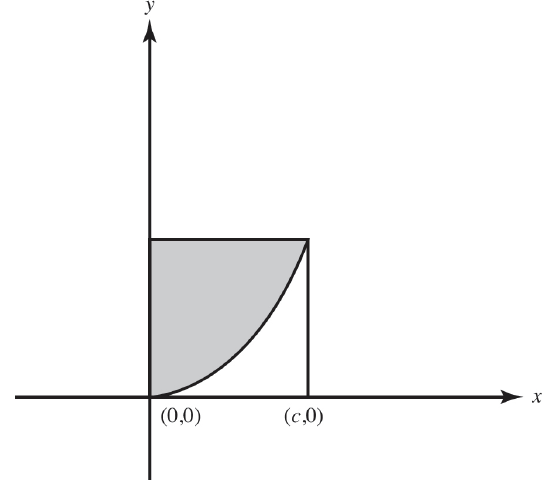
\includegraphics[width=0.6\linewidth]{data/calculus-figures/c7-a15.png}\end{center}
\begin{list}{}{\setlength{\leftmargin}{3em}\setlength{\labelwidth}{2.5em}\setlength{\itemsep}{0pt}\setlength{\topsep}{2pt}}
\item[(A)] $3:4$
\item[(B)] $5:4$
\item[(C)] $4:3$
\item[(D)] $3:1$
\end{list}

\bigskip\noindent\textbf{A16.}\ Find the volume when the region bounded by $y=x^2$, $x=2$, and $y=0$ rotates about the $x$-axis.
\begin{list}{}{\setlength{\leftmargin}{3em}\setlength{\labelwidth}{2.5em}\setlength{\itemsep}{0pt}\setlength{\topsep}{2pt}}
\item[(A)] $64\pi/3$
\item[(B)] $8\pi$
\item[(C)] $8\pi/3$
\item[(D)] $32\pi/5$
\end{list}

\bigskip\noindent\textbf{A17.}\ Find the volume when the region bounded by $y=x^2$, $x=2$, and $y=0$ rotates about the $y$-axis.
\begin{list}{}{\setlength{\leftmargin}{3em}\setlength{\labelwidth}{2.5em}\setlength{\itemsep}{0pt}\setlength{\topsep}{2pt}}
\item[(A)] $16\pi/3$
\item[(B)] $4\pi$
\item[(C)] $32\pi/5$
\item[(D)] $8\pi$
\end{list}

\bigskip\noindent\textbf{A18.}\ Find the volume when the first-quadrant region bounded by $y=x^2$, the $y$-axis, and $y=4$ rotates about the $y$-axis.
\begin{list}{}{\setlength{\leftmargin}{3em}\setlength{\labelwidth}{2.5em}\setlength{\itemsep}{0pt}\setlength{\topsep}{2pt}}
\item[(A)] $8\pi$
\item[(B)] $4\pi$
\item[(C)] $32\pi/3$
\item[(D)] $16\pi/3$
\end{list}

\bigskip\noindent\textbf{A19.}\ Find the volume when the region between $y=x^2$ and $y=4$ rotates about the $x$-axis.
\begin{list}{}{\setlength{\leftmargin}{3em}\setlength{\labelwidth}{2.5em}\setlength{\itemsep}{0pt}\setlength{\topsep}{2pt}}
\item[(A)] $64\pi/5$
\item[(B)] $512\pi/15$
\item[(C)] $256\pi/5$
\item[(D)] $128\pi/5$
\end{list}

\bigskip\noindent\textbf{A20.}\ Find the volume when the region between $y=x^2$ and $y=4$ rotates about $y=4$.
\begin{list}{}{\setlength{\leftmargin}{3em}\setlength{\labelwidth}{2.5em}\setlength{\itemsep}{0pt}\setlength{\topsep}{2pt}}
\item[(A)] $256\pi/15$
\item[(B)] $256\pi/5$
\item[(C)] $512\pi/5$
\item[(D)] $512\pi/15$
\end{list}

\bigskip\noindent\textbf{A21.}\ Find the volume when one arch of $y=\sin x$ and the $x$-axis rotates about the $x$-axis.
\begin{list}{}{\setlength{\leftmargin}{3em}\setlength{\labelwidth}{2.5em}\setlength{\itemsep}{0pt}\setlength{\topsep}{2pt}}
\item[(A)] $\tfrac\pi2(\pi-\tfrac12)$
\item[(B)] $\pi^2/2$
\item[(C)] $\pi^2/4$
\item[(D)] $\pi^2$
\end{list}

\bigskip\noindent\textbf{A22.}\ Find the volume when the trapezoid with vertices $(2,0),(2,2),(4,0),(4,4)$ rotates about the $x$-axis.
\begin{list}{}{\setlength{\leftmargin}{3em}\setlength{\labelwidth}{2.5em}\setlength{\itemsep}{0pt}\setlength{\topsep}{2pt}}
\item[(A)] $56\pi/3$
\item[(B)] $128\pi/3$
\item[(C)] $92\pi/3$
\item[(D)] $112\pi/3$
\end{list}

\bigskip\noindent\textbf{A23.}\ A solid has a circular base of radius $a$, centered at the origin. Cross sections perpendicular to the $x$-axis are squares. Find its volume.
\begin{list}{}{\setlength{\leftmargin}{3em}\setlength{\labelwidth}{2.5em}\setlength{\itemsep}{0pt}\setlength{\topsep}{2pt}}
\item[(A)] $8a^3/3$
\item[(B)] $2\pi a^3$
\item[(C)] $4\pi a^3$
\item[(D)] $16a^3/3$
\end{list}

\bigskip\noindent\textbf{A24.}\ A solid has base bounded by $x^2=8y$ and $y=4$. Cross sections perpendicular to the $y$-axis are equilateral triangles. Find its volume.
\begin{list}{}{\setlength{\leftmargin}{3em}\setlength{\labelwidth}{2.5em}\setlength{\itemsep}{0pt}\setlength{\topsep}{2pt}}
\item[(A)] $64\sqrt3/3$
\item[(B)] $64\sqrt3$
\item[(C)] $32\sqrt3$
\item[(D)] $32$
\end{list}

\bigskip\noindent\textbf{A25.}\ A solid has base bounded by $y=e^{-x}$, the coordinate axes, and $x=1$. Cross sections perpendicular to the $x$-axis are squares. Find its volume.
\begin{list}{}{\setlength{\leftmargin}{3em}\setlength{\labelwidth}{2.5em}\setlength{\itemsep}{0pt}\setlength{\topsep}{2pt}}
\item[(A)] $e^2-1$
\item[(B)] $1-e^{-2}$
\item[(C)] $(e^2-1)/2$
\item[(D)] $\tfrac12(1-e^{-2})$
\end{list}

\bigskip\noindent\textbf{A26.}\ Find the length of the curve $y^2=x^3$ cut off by $x=4$.
\begin{center}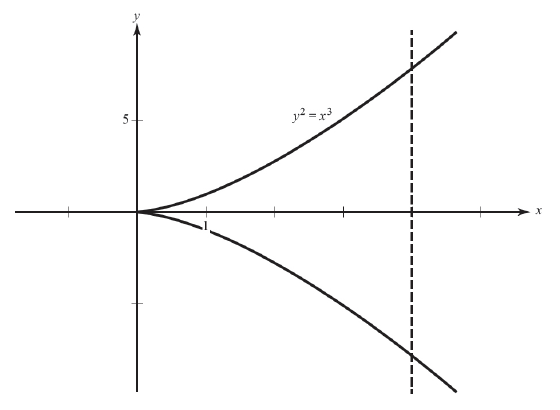
\includegraphics[width=0.6\linewidth]{data/calculus-figures/c7-a26.png}\end{center}
\begin{list}{}{\setlength{\leftmargin}{3em}\setlength{\labelwidth}{2.5em}\setlength{\itemsep}{0pt}\setlength{\topsep}{2pt}}
\item[(A)] $\tfrac43(10\sqrt{10}-1)$
\item[(B)] $\tfrac8{27}(10^{3/2}-1)$
\item[(C)] $\tfrac{16}{27}(10^{3/2}-1)$
\item[(D)] $\tfrac{16}{27}10\sqrt{10}$
\end{list}

\bigskip\noindent\textbf{A27.}\ The length of $y=\ln(\cos x)$ from $x=\pi/4$ to $x=\pi/3$ equals
\begin{list}{}{\setlength{\leftmargin}{3em}\setlength{\labelwidth}{2.5em}\setlength{\itemsep}{0pt}\setlength{\topsep}{2pt}}
\item[(A)] $\int_{\pi/4}^{\pi/3}\sqrt{1+\tan^2x}\,dx$
\item[(B)] $\int_{\pi/4}^{\pi/3}\sqrt{1+(\ln(\cos x))^2}\,dx$
\item[(C)] $\int_{\pi/4}^{\pi/3}\sqrt{1+1/\cos^2x}\,dx$
\item[(D)] $\int_{\pi/4}^{\pi/3}\sqrt{1+\cot^2x}\,dx$
\end{list}

\bigskip\noindent\textbf{A28.}\ $\int_0^\infty e^{-x}\,dx=$
\begin{list}{}{\setlength{\leftmargin}{3em}\setlength{\labelwidth}{2.5em}\setlength{\itemsep}{0pt}\setlength{\topsep}{2pt}}
\item[(A)] $1$
\item[(B)] $1/e$
\item[(C)] $-1$
\item[(D)] divergent
\end{list}

\bigskip\noindent\textbf{A29.}\ $\int_0^e du/u=$
\begin{list}{}{\setlength{\leftmargin}{3em}\setlength{\labelwidth}{2.5em}\setlength{\itemsep}{0pt}\setlength{\topsep}{2pt}}
\item[(A)] $1$
\item[(B)] $1/e$
\item[(C)] $-1/e^2$
\item[(D)] divergent
\end{list}

\bigskip\noindent\textbf{A30.}\ $\int_1^2(t-1)^{-1/3}\,dt=$
\begin{list}{}{\setlength{\leftmargin}{3em}\setlength{\labelwidth}{2.5em}\setlength{\itemsep}{0pt}\setlength{\topsep}{2pt}}
\item[(A)] $2/3$
\item[(B)] $3/2$
\item[(C)] $3$
\item[(D)] divergent
\end{list}

\bigskip\noindent\textbf{A31.}\ $\int_2^4(x-3)^{-2/3}\,dx=$
\begin{list}{}{\setlength{\leftmargin}{3em}\setlength{\labelwidth}{2.5em}\setlength{\itemsep}{0pt}\setlength{\topsep}{2pt}}
\item[(A)] $6$
\item[(B)] $0$
\item[(C)] $2/3$
\item[(D)] divergent
\end{list}

\bigskip\noindent\textbf{A32.}\ $\int_2^4(x-3)^{-2}\,dx=$
\begin{list}{}{\setlength{\leftmargin}{3em}\setlength{\labelwidth}{2.5em}\setlength{\itemsep}{0pt}\setlength{\topsep}{2pt}}
\item[(A)] $2$
\item[(B)] $-2$
\item[(C)] $0$
\item[(D)] divergent
\end{list}

\bigskip\noindent\textbf{A33.}\ $\int_0^{\pi/2}\frac{\sin x}{\sqrt{1-\cos x}}\,dx=$
\begin{list}{}{\setlength{\leftmargin}{3em}\setlength{\labelwidth}{2.5em}\setlength{\itemsep}{0pt}\setlength{\topsep}{2pt}}
\item[(A)] $-2$
\item[(B)] $1/2$
\item[(C)] $2$
\item[(D)] divergent
\end{list}

\bigskip\noindent\textbf{A34.}\ Find the first-quadrant area under $y=e^{-x}$.
\begin{list}{}{\setlength{\leftmargin}{3em}\setlength{\labelwidth}{2.5em}\setlength{\itemsep}{0pt}\setlength{\topsep}{2pt}}
\item[(A)] $1$
\item[(B)] $e$
\item[(C)] $1/e$
\item[(D)] divergent
\end{list}

\bigskip\noindent\textbf{A35.}\ Find the first-quadrant area under $y=xe^{-x^2}$.
\begin{center}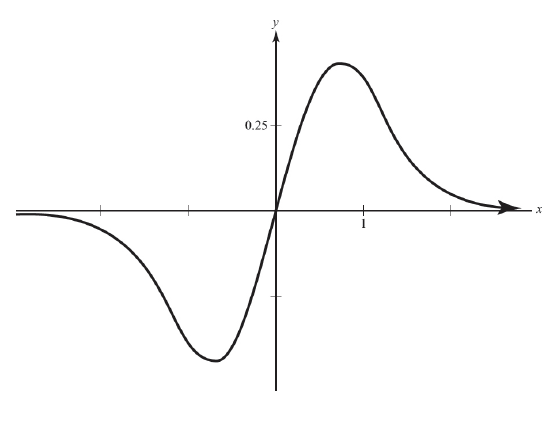
\includegraphics[width=0.6\linewidth]{data/calculus-figures/c7-a35.png}\end{center}
\begin{list}{}{\setlength{\leftmargin}{3em}\setlength{\labelwidth}{2.5em}\setlength{\itemsep}{0pt}\setlength{\topsep}{2pt}}
\item[(A)] $2$
\item[(B)] $2/e$
\item[(C)] $1/2$
\item[(D)] divergent
\end{list}

\bigskip\noindent\textbf{A36.}\ Find the first-quadrant area above $y=1$, between the $y$-axis and $y=1/x$.
\begin{list}{}{\setlength{\leftmargin}{3em}\setlength{\labelwidth}{2.5em}\setlength{\itemsep}{0pt}\setlength{\topsep}{2pt}}
\item[(A)] $1$
\item[(B)] $2$
\item[(C)] $1/2$
\item[(D)] divergent
\end{list}

\bigskip\noindent\textbf{A37.}\ Find the area between $y=4/(1+x^2)$ and the $x$-axis.
\begin{center}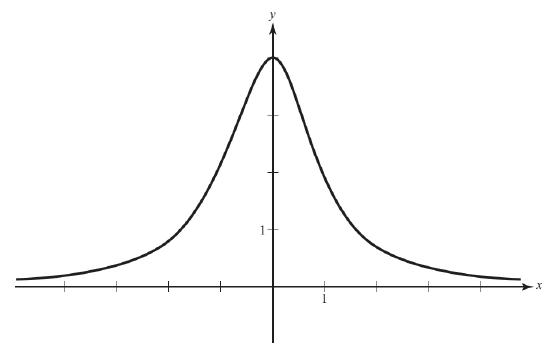
\includegraphics[width=0.6\linewidth]{data/calculus-figures/c7-a37.png}\end{center}
\begin{list}{}{\setlength{\leftmargin}{3em}\setlength{\labelwidth}{2.5em}\setlength{\itemsep}{0pt}\setlength{\topsep}{2pt}}
\item[(A)] $2\pi$
\item[(B)] $4\pi$
\item[(C)] $8\pi$
\item[(D)] divergent
\end{list}

\bigskip\noindent\textbf{A38.}\ Find the area above the $x$-axis, between $y=4/\sqrt{1-x^2}$ and its asymptotes.
\begin{center}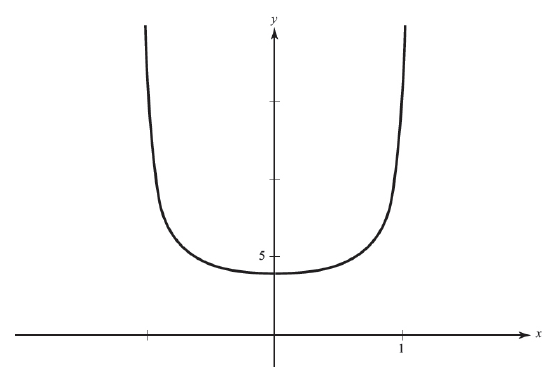
\includegraphics[width=0.6\linewidth]{data/calculus-figures/c7-a38.png}\end{center}
\begin{list}{}{\setlength{\leftmargin}{3em}\setlength{\labelwidth}{2.5em}\setlength{\itemsep}{0pt}\setlength{\topsep}{2pt}}
\item[(A)] $\pi$
\item[(B)] $2\pi$
\item[(C)] $4\pi$
\item[(D)] divergent
\end{list}

\bigskip\noindent\textbf{A39.}\ Find the volume generated by rotating the region under $y=1/x$, to the right of $x=1$, and above $y=0$ about the $x$-axis.
\begin{list}{}{\setlength{\leftmargin}{3em}\setlength{\labelwidth}{2.5em}\setlength{\itemsep}{0pt}\setlength{\topsep}{2pt}}
\item[(A)] $\pi/2$
\item[(B)] $\pi$
\item[(C)] $2\pi$
\item[(D)] divergent
\end{list}

\bigskip\noindent\textbf{A40.}\ Find the volume generated by rotating the first-quadrant region under $y=e^{-x}$ about the $x$-axis.
\begin{list}{}{\setlength{\leftmargin}{3em}\setlength{\labelwidth}{2.5em}\setlength{\itemsep}{0pt}\setlength{\topsep}{2pt}}
\item[(A)] $\pi/2$
\item[(B)] $\pi$
\item[(C)] $2\pi$
\item[(D)] divergent
\end{list}

\bigskip\noindent\textbf{B1.}\ The area between $y=2-x^2$ and $y=x-4$ is given by
\begin{list}{}{\setlength{\leftmargin}{3em}\setlength{\labelwidth}{2.5em}\setlength{\itemsep}{0pt}\setlength{\topsep}{2pt}}
\item[(A)] $\int_{-2}^3(6-x-x^2)\,dx$
\item[(B)] $\int_{-2}^1(2+x+x^2)\,dx$
\item[(C)] $\int_{-3}^2(6-x-x^2)\,dx$
\item[(D)] $2\int_0^{\sqrt2}(2-x^2)\,dx+\int_{-3}^2(4-x)\,dx$
\end{list}

\bigskip\noindent\textbf{B2.}\ For continuous $f$ on $[1,8]$, the table is $\begin{array}{c|ccccc}x&1&2&5&6&8\\\hline f(x)&1.62&4.15&7.5&9.0&12.13\end{array}$. Use four trapezoids to approximate the area under the curve from $1$ to $8$, to two decimal places.
\begin{list}{}{\setlength{\leftmargin}{3em}\setlength{\labelwidth}{2.5em}\setlength{\itemsep}{0pt}\setlength{\topsep}{2pt}}
\item[(A)] $24.87$
\item[(B)] $39.57$
\item[(C)] $49.74$
\item[(D)] $59.91$
\end{list}

\bigskip\noindent\textbf{B3.}\ Find the area enclosed by the four-leaved rose $r=\cos2\theta$, to three decimal places.
\begin{list}{}{\setlength{\leftmargin}{3em}\setlength{\labelwidth}{2.5em}\setlength{\itemsep}{0pt}\setlength{\topsep}{2pt}}
\item[(A)] $0.785$
\item[(B)] $1.571$
\item[(C)] $3.142$
\item[(D)] $6.283$
\end{list}

\bigskip\noindent\textbf{B4.}\ The area of the small loop of $r=1-2\sin\theta$ is given by
\begin{list}{}{\setlength{\leftmargin}{3em}\setlength{\labelwidth}{2.5em}\setlength{\itemsep}{0pt}\setlength{\topsep}{2pt}}
\item[(A)] $\int_{\pi/3}^{5\pi/3}[\tfrac12(1-2\sin\theta)]^2\,d\theta$
\item[(B)] $\int_{7\pi/6}^{3\pi/2}(1-2\sin\theta)^2\,d\theta$
\item[(C)] $\int_{\pi/6}^{\pi/2}(1-2\sin\theta)^2\,d\theta$
\item[(D)] $\int_0^{\pi/6}[\tfrac12(1-2\sin\theta)]^2\,d\theta+\int_{5\pi/6}^{\pi}[\tfrac12(1-2\sin\theta)]^2\,d\theta$
\end{list}

\bigskip\noindent\textbf{B5.}\ Find the volume generated by rotating the region between $y=x^2$ and $y=4$ about $y=-1$.
\begin{list}{}{\setlength{\leftmargin}{3em}\setlength{\labelwidth}{2.5em}\setlength{\itemsep}{0pt}\setlength{\topsep}{2pt}}
\item[(A)] $4\pi\int_{-1}^4(y+1)\sqrt y\,dy$
\item[(B)] $2\pi\int_0^2(4-x^2)^2\,dx$
\item[(C)] $\pi\int_{-2}^2(16-x^4)\,dx$
\item[(D)] $2\pi\int_0^2(24-2x^2-x^4)\,dx$
\end{list}

\bigskip\noindent\textbf{B6.}\ Find the volume generated by rotating the region between $y=3x-x^2$ and $y=0$ about the $x$-axis.
\begin{list}{}{\setlength{\leftmargin}{3em}\setlength{\labelwidth}{2.5em}\setlength{\itemsep}{0pt}\setlength{\topsep}{2pt}}
\item[(A)] $\pi\int_0^3(9x^2+x^4)\,dx$
\item[(B)] $\pi\int_0^3(3x-x^2)^2\,dx$
\item[(C)] $\pi\int_0^{\sqrt3}(3x-x^2)\,dx$
\item[(D)] $2\pi\int_0^3y\sqrt{9-4y}\,dy$
\end{list}

\bigskip\noindent\textbf{B7.}\ Find the volume generated by rotating the region between $y=3x-x^2$ and $y=x$ about the $x$-axis.
\begin{list}{}{\setlength{\leftmargin}{3em}\setlength{\labelwidth}{2.5em}\setlength{\itemsep}{0pt}\setlength{\topsep}{2pt}}
\item[(A)] $\pi\int_0^{3/2}[(3x-x^2)^2-x^2]\,dx$
\item[(B)] $\pi\int_0^2(9x^2-6x^3)\,dx$
\item[(C)] $\pi\int_0^2[(3x-x^2)^2-x^2]\,dx$
\item[(D)] $\pi\int_0^3(2x-x^2)^2\,dx$
\end{list}

\bigskip\noindent\textbf{B8.}\ Find the volume generated by rotating the region bounded by $y=\ln x$, $y=0$, and $x=e$ about $x=e$.
\begin{list}{}{\setlength{\leftmargin}{3em}\setlength{\labelwidth}{2.5em}\setlength{\itemsep}{0pt}\setlength{\topsep}{2pt}}
\item[(A)] $\pi\int_1^e(e-x)\ln x\,dx$
\item[(B)] $\pi\int_0^1(e-e^y)^2\,dy$
\item[(C)] $2\pi\int_1^e(e-\ln x)\,dx$
\item[(D)] $\pi\int_0^e(e^2-2e^{y+1}+e^{2y})\,dy$
\end{list}

\bigskip\noindent\textbf{B9.}\ A sphere of radius $r$ is cut by a plane at distance $h$ from the center, where $0<h<r$. Find the smaller part's volume.
\begin{list}{}{\setlength{\leftmargin}{3em}\setlength{\labelwidth}{2.5em}\setlength{\itemsep}{0pt}\setlength{\topsep}{2pt}}
\item[(A)] $\tfrac\pi3(2r^3+h^3-3r^2h)$
\item[(B)] $\tfrac{\pi h}3(3r^2-h^2)$
\item[(C)] $\tfrac43\pi r^3+\tfrac{h^3}3-r^2h$
\item[(D)] $\tfrac\pi3(2r^3+3r^2h-h^3)$
\end{list}

\bigskip\noindent\textbf{B10.}\ If $f$ and $g$ intersect at $a,b$ and $f(x)>g(x)>0$ on $(a,b)$, find the volume generated by rotating their enclosed region about the $x$-axis.
\begin{list}{}{\setlength{\leftmargin}{3em}\setlength{\labelwidth}{2.5em}\setlength{\itemsep}{0pt}\setlength{\topsep}{2pt}}
\item[(A)] $\pi\int_a^bf(x)^2\,dx-\int_a^bg(x)^2\,dx$
\item[(B)] $\pi\int_a^b[f(x)-g(x)]^2\,dx$
\item[(C)] $2\pi\int_a^bx[f(x)-g(x)]\,dx$
\item[(D)] $\pi\int_a^b[f(x)^2-g(x)^2]\,dx$
\end{list}

\bigskip\noindent\textbf{B11.}\ The length of one arch of $x=t-\sin t$, $y=1-\cos t$ equals
\begin{list}{}{\setlength{\leftmargin}{3em}\setlength{\labelwidth}{2.5em}\setlength{\itemsep}{0pt}\setlength{\topsep}{2pt}}
\item[(A)] $\int_0^\pi\sqrt{1-\cos t}\,dt$
\item[(B)] $\int_0^{2\pi}\sqrt{(1-\cos t)/2}\,dt$
\item[(C)] $\int_0^\pi\sqrt{2-2\cos t}\,dt$
\item[(D)] $\int_0^{2\pi}\sqrt{2-2\cos t}\,dt$
\end{list}

\bigskip\noindent\textbf{B12.}\ The length of $4x=y^2$ cut off by $x=2$ is given by
\begin{list}{}{\setlength{\leftmargin}{3em}\setlength{\labelwidth}{2.5em}\setlength{\itemsep}{0pt}\setlength{\topsep}{2pt}}
\item[(A)] $\int_{-1}^1\sqrt{x^2+1}\,dx$
\item[(B)] $\tfrac12\int_0^2\sqrt{4+y^2}\,dy$
\item[(C)] $\int_{-1}^1\sqrt{1+x}\,dx$
\item[(D)] $\int_0^{2\sqrt2}\sqrt{4+y^2}\,dy$
\end{list}

\bigskip\noindent\textbf{B13.}\ Find the length of $x=e^t\cos t$, $y=e^t\sin t$ for $2\le t\le3$.
\begin{list}{}{\setlength{\leftmargin}{3em}\setlength{\labelwidth}{2.5em}\setlength{\itemsep}{0pt}\setlength{\topsep}{2pt}}
\item[(A)] $17.956$
\item[(B)] $25.393$
\item[(C)] $26.413$
\item[(D)] $37.354$
\end{list}

\bigskip\noindent\textbf{B14.}\ Which integral is improper?
\begin{list}{}{\setlength{\leftmargin}{3em}\setlength{\labelwidth}{2.5em}\setlength{\itemsep}{0pt}\setlength{\topsep}{2pt}}
\item[(A)] $\int_0^2\frac{dx}{\sqrt{x+1}}$
\item[(B)] $\int_{-1}^1\frac{dx}{1+x^2}$
\item[(C)] $\int_0^2\frac{x\,dx}{1-x^2}$
\item[(D)] $\int_0^{\pi/3}\frac{\sin x\,dx}{\cos^2x}$
\end{list}

\bigskip\noindent\textbf{B15.}\ Which improper integral diverges?
\begin{list}{}{\setlength{\leftmargin}{3em}\setlength{\labelwidth}{2.5em}\setlength{\itemsep}{0pt}\setlength{\topsep}{2pt}}
\item[(A)] $\int_1^\infty x^{-2}\,dx$
\item[(B)] $\int_0^\infty e^{-x}\,dx$
\item[(C)] $\int_{-1}^1\frac{dx}{\sqrt[3]x}$
\item[(D)] $\int_{-1}^1x^{-2}\,dx$
\end{list}

\bigskip\noindent\textbf{B16.}\ Which improper integral diverges?
\begin{list}{}{\setlength{\leftmargin}{3em}\setlength{\labelwidth}{2.5em}\setlength{\itemsep}{0pt}\setlength{\topsep}{2pt}}
\item[(A)] $\int_0^\infty\frac{dx}{1+x^2}$
\item[(B)] $\int_0^1x^{-1/3}\,dx$
\item[(C)] $\int_0^\infty\frac{dx}{e^x+2}$
\item[(D)] $\int_0^\infty x^{-1/3}\,dx$
\end{list}

\end{document}
